\scanpage{19}
de Kostant. On a donc
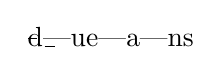
\begin{tikzpicture}[baseline=(w.base)]
\node[inner sep=0pt] (w) {\unsure{d|u}\unsure{e|a|n}s};
\draw[line width=.3pt] ([xshift=.04em,yshift=.72ex]w.base west)--++(.32em,0);
\draw[line width=.3pt] ([xshift=.63em,yshift=.02ex]w.base west)--++(.38em,0);
\end{tikzpicture}
morphismes $f\handwritten{\unsure{\mathrel{\mapstochar\relbar}|\mapsto}}f\handwritten{\circ}i_o$ et $f\handwritten{\mapsto}f(u_o)$ de $\operatorname{Dyn}_c$ dans $\operatorname{ST}_c$ resp. $\operatorname{Un}_c$. D'autre part, Deligne nous fournit $\operatorname{Un}_c\handwritten{\to\underline{\varnothing}}_c$, et celui-ci peut aussi être défini par la commutativité du diagramme \handwritten{d'esp. homogènes}
\diagram{\begin{tikzcd}[ampersand replacement=\&,column sep=large,row sep=large]
\operatorname{ST}_c\handwritten{\simeq}(\operatorname{CL})_{c'}
\handwritten{\arrow[d]}
\arrow[d,draw=gray!45,-,to path={([xshift=-.25ex,yshift=.45ex]\tikztotarget.north) .. controls +(0,-.65ex) and +(0,-.65ex) .. ([xshift=.25ex,yshift=.45ex]\tikztotarget.north)}]
\arrow[d,phantom,"{\unsure{}}" description,near end]
\& \operatorname{Dyn}_c \handwritten{\arrow[l]} \handwritten{\arrow[d]} \\
\handwritten{\underline{\varnothing}}_c\handwritten{\simeq}\operatorname{Par}_{c'} \& \operatorname{Un}_c \handwritten{\arrow[l]}
\end{tikzcd}}
\margin{\handwritten{\diagram{\begin{tikzcd}[ampersand replacement=\&,column sep=small,row sep=small]
L \arrow[d] \&
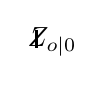
\begin{tikzpicture}[baseline=(z.base)]
\node[inner sep=0pt] (z) {$\unsure{Z}_{\unsure{o|0}}$};
\draw[line width=1pt] ([xshift=.35em,yshift=-.1ex]z.base west)--++(0,1.45ex);
\end{tikzpicture}
\arrow[l] \arrow[d] \\
P \& \unsure{\mathfrak{z}|z|Z}(\unsure{\cdot}e) \arrow[l]
\end{tikzcd}}}}
.

Pour qu'il existe un point rationnel de \deleted{$\operatorname{Dyn}_c$, ou ce qui revient au même} $\handwritten{\unsure{\underline{\varnothing}|\underline{\phi}}}_c\handwritten{\simeq}\operatorname{Par}_{c'}$, il faut (et suffit) qu'il en existe un de $\operatorname{Dy}\unsure{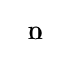
\begin{tikzpicture}[baseline=(n.base)]\node[inner sep=0pt] (n) {$\mathrm n$};\node[inner sep=0pt] at ([xshift=.02em,yshift=-.02ex]n.center) {$\mathrm o$};\end{tikzpicture}}_c$ \deleted{i.e. que $G$ soit quasi-déployé;}\inserted{\handwritten{(i.e., si $Z_o=e$, que $G$ est quasi-déployé)}}\handwritten{:} en effet, $P$ étant choisi, \deleted{les $i$}\begin{tikzpicture}[baseline=-.1ex]\draw[line width=.3pt](0,0)--(.48em,.8ex);\draw[line width=.3pt](0,.8ex)--(.48em,0);\end{tikzpicture} on peut en choisir un \deleted{point rationnel} sous-groupe de Lévi
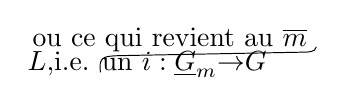
\begin{tikzpicture}[baseline=(lev.base)]
\node[inner sep=0pt,anchor=base west] (lev) at (0,0) {$L$,\deleted{i.e}. un $i:\underline{G}_m\handwritten{\to}G$};
\node[inner sep=0pt,anchor=south west] at (.18em,1.55ex) {\inserted{\handwritten{ou ce qui revient au $\overline{m}$}}};
\draw[line width=.35pt] (2.65em,-.15ex) .. controls (2.58em,1.15ex) and (2.75em,1.2ex) .. (3.3em,1.25ex) -- (10.1em,1.55ex) .. controls (10.4em,1.6ex) and (10.45em,1.8ex) .. (10.45em,2.0ex);
\end{tikzpicture}
dans la classe $c$,définissant $P$, et alors les $u=\exp(e)$ qui \deleted{aux} s'adaptent à $i$ forment un ouvert dense de $\handwritten{\unsure{\mathfrak{g}|\mathscr{G}}(2)}$, qui \deleted{est donc non vide} a donc un point rationnel. On voit donc que pour certaines classes de paraboliques (qu'on pourrait appeler les paraboliques de
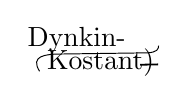
\begin{tikzpicture}[baseline=(kos.base)]
\node[inner sep=0pt,anchor=base west] (kos) at (0,0) {Kostant\handwritten{\unsure{)}}};
\node[inner sep=0pt,anchor=south west] at (-.7em,1.4ex) {\inserted{Dynkin-}};
\draw[line width=.35pt] (-.25em,-.15ex) .. controls (-.6em,1.15ex) and (-.05em,1.3ex) .. (.55em,1.3ex) -- (3.65em,1.4ex) .. controls (4em,1.45ex) and (4.05em,1.7ex) .. (4.05em,2.0ex);
\draw[line width=.65pt] ([xshift=-.52em,yshift=.4ex]kos.base east)--++(.65em,.03ex);
\end{tikzpicture}
l'existence d'un parabolique de cette classe rationnel sur $k$ implique déjà que $G$ est quasi-déployé. (NB Quand $G$ n'est pas une forme intérieure, il faut faire attention cependant de vérifier d'abord que la classe $c'$ de $P$ provient bien d'un $c$ de Dynkin \uline{invariant par} $\handwritten{\Gamma}$, et il n'est pas clair que cette propriété

\begin{tikzpicture}[baseline=(res.base)]
\node[inner sep=0pt,anchor=base west] (res) at (0,0) {résulte};
\node[inner sep=0pt,anchor=south west] at (-.1em,1.4ex) {\inserted{de $c$}};
\draw[line width=.35pt] (-.3em,-.18ex) .. controls (-.35em,1.1ex) and (0,1.2ex) .. (.65em,1.2ex) -- (2.1em,1.25ex) .. controls (2.5em,1.3ex) and (2.7em,1.5ex) .. (2.7em,1.9ex);
\end{tikzpicture}
du fait que $c'$ est \unsure{invariantè|invariante} par $\handwritten{\Gamma}$, faute de savoir si $c\handwritten{\mapsto}c'$ est injectif sur les classes de Dynkin). \handwritten{(}On notera aussi que l'argument donné
\unsure{
\begin{tikzpicture}[baseline=(m.base)]\node[inner sep=0pt] (m) {m};\node[inner sep=0pt] at ([xshift=.01em,yshift=-.01ex]m.center) {p};\end{tikzpicture}}arche
également sur un anneau semi-local (de car. nulle jusqu'à nouvel ordre).\handwritten{)}
\margin{\handwritten{\scriptsize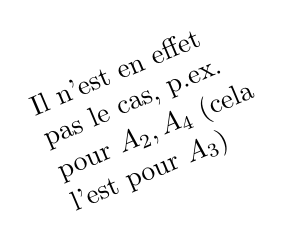
\begin{tikzpicture}[rotate=23,transform shape]
\node[inner sep=0pt,anchor=west] at (0,1.35) {Il n'est en effet};
\node[inner sep=0pt,anchor=west] at (0,.9) {pas le cas, p.ex.};
\node[inner sep=0pt,anchor=west] at (0,.45) {pour $A_2,A_4$ (cela};
\node[inner sep=0pt,anchor=west] at (0,0) {l'est pour $A_3$)};
\end{tikzpicture}}}
% slanted margin note
Ceci montre l'intérêt, pour des questions arithmétiques, de déterminer exactement les

\begin{tikzpicture}[baseline=(sg.base)]
\node[inner sep=0pt,anchor=base west] (sg) at (0,0) {sous-groupes};
\node[inner sep=0pt,anchor=south west] at (-.35em,1.4ex) {\inserted{classes\,\raisebox{.45ex}{\handwritten{de}}}};
\draw[line width=.35pt] (-.3em,-.12ex) .. controls (-.25em,.9ex) and (.4em,1.25ex) .. (1.1em,1.2ex) .. controls (2em,1.05ex) and (3.05em,1.05ex) .. (3.3em,1.8ex);
\end{tikzpicture}
parab\handwritten{\unsure{\begin{tikzpicture}[baseline=-.1ex]\draw[line width=.45pt](0,0)--(.42em,.32ex);\draw[line width=.2pt,gray!50](.05em,.35ex)--(.42em,.85ex);\end{tikzpicture}}}oliques de Dynkin-Kostant des divers groupes simples, et de voir si\unsure{:|''} leur stabilisateur dans $\operatorname{Autext}(G_o)$ est le même que celui des $c$ de Dynkin correspondants, et pas str. plus grand.

On notera cependant que si une filtration du foncteur \deleted{fib} oubli peut être définie par un élément unipotent, la classe de conjugaison de ce der-
% archive sheet number: 18
